\chapter{The CLI-Tutor Tool}
% - Tool (CLI-Tutor)
%   - overview
%       - cirriculum
%       - lesson design
%            - deliberate emphasis on  easy vocabulary
%       - usability considerations
%       - safety considerations
%   - web version
%
\label{chap:clitutor}

\begin{lstlisting}[float=htbp, keepspaces, frame=single, language={}, caption=Output of the help flag of \textit{CLI-Tutor} running in a docker container.]

cli-student@3bc86f9090f9:~/tutor$ cli-tutor -h

        _ _       __        __
  _____/ (_)     / /___  __/ /_____  _____
 / ___/ / /_____/ __/ / / / __/ __ \/ ___/
/ /__/ / /_____/ /_/ /_/ / /_/ /_/ / /
\___/_/_/      \__/\__,_/\__/\____/_/

A simple command line tutor application that aims to introduce users to the
    basics of command line interaction.
    Web version is available at https://clitutor.chistole.ch

Usage:
  cli-tutor [flags]
  cli-tutor [command]

Available Commands:
  completion  Generate the autocompletion script for the specified shell
  help        Help about any command
  info        Prints information about the tool and log collection
  repo        Prints a url to the git repository for this tool
  version     Print the version number of cli-tutor

Flags:
  -h, --help            help for cli-tutor
  -n, --no-upload-log   Do not send a copy of the log to the developer
  -x, --no-welcome      Do not show welcome message when entering tutor

Use "cli-tutor [command] --help" for more information about a command.
\end{lstlisting}


The \textit{CLI-Tutor} tool is a command line application written in the Go programming language. 


\section{Overview}
\subsection{Curriculum}
\subsection{Lesson Design}
\subsection{Usability Considerations}
\subsection{Safety Considerations}
\section{Web Version}


\begin{figure}[htbp]
    \centering
    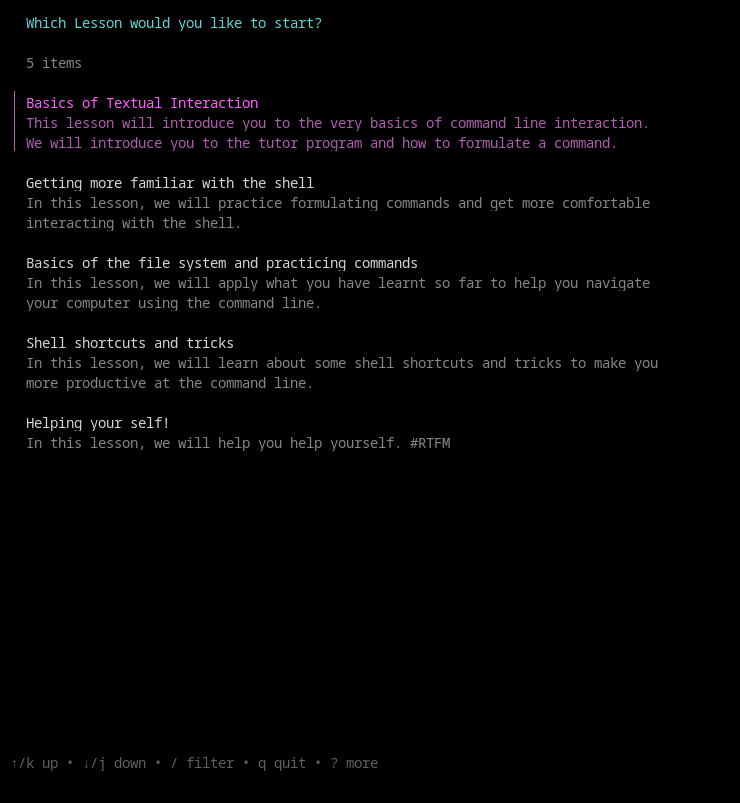
\includegraphics[width=0.8\textwidth]{img/climenu}
    \caption{Screen shot of \textit{CLI-Tutor} menu screen.}
    \label{fig:clitutormenu}
\end{figure}
\begin{figure}[htbp]
	\centering
	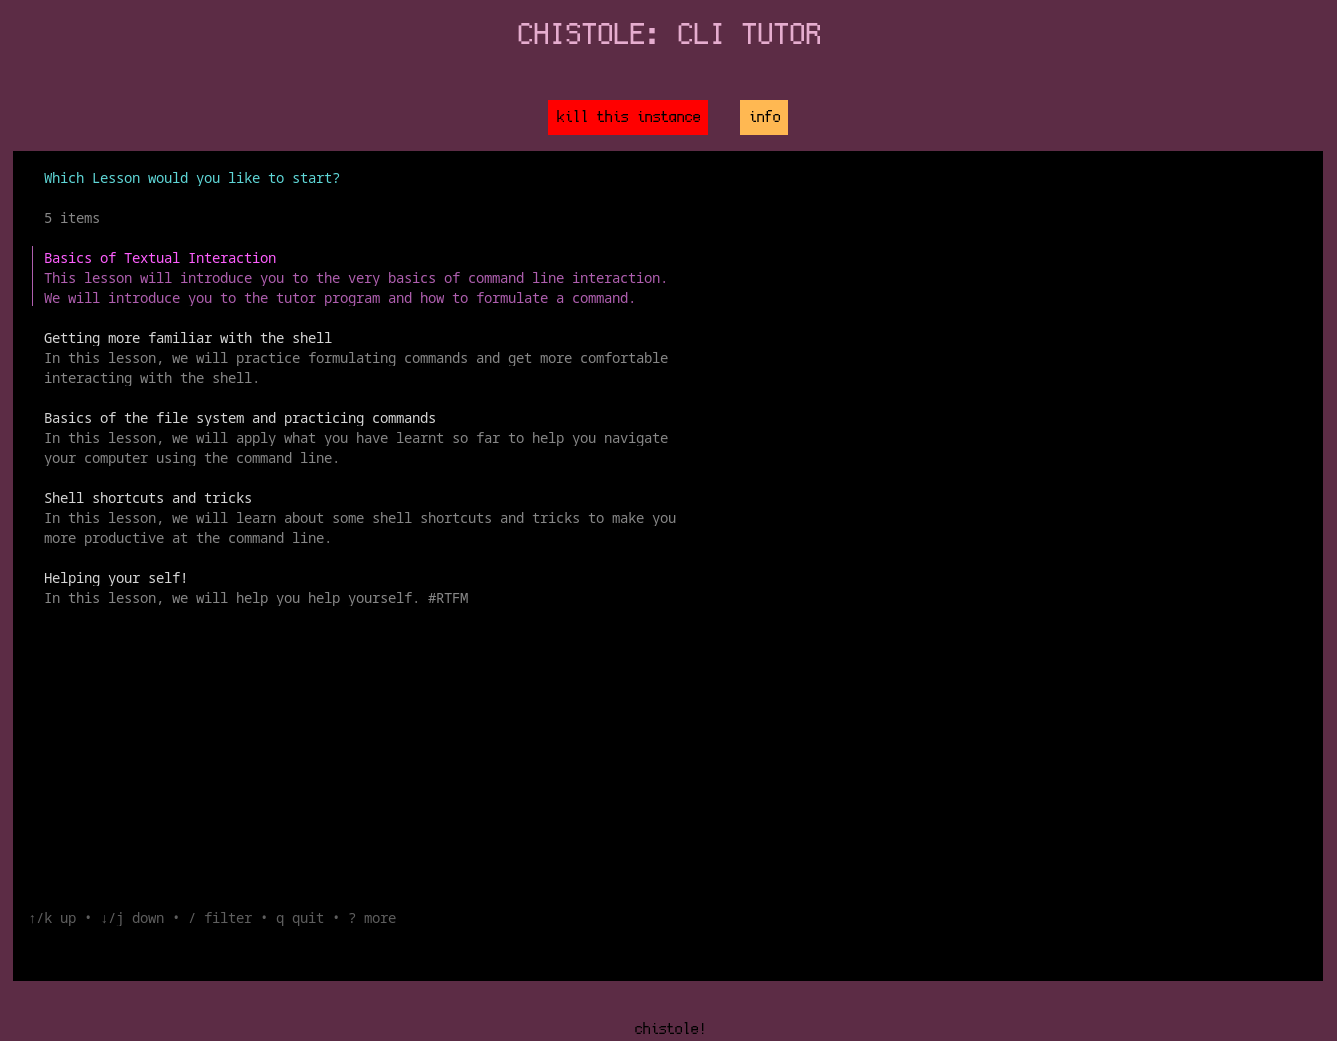
\includegraphics[width=1\textwidth]{img/cliwebfull}
	\caption{Screen shot of \textit{CLI-Tutor} menu screen in the web version.}
	\label{fig:webversion}
\end{figure}

\begin{figure}[htbp]
	\centering
	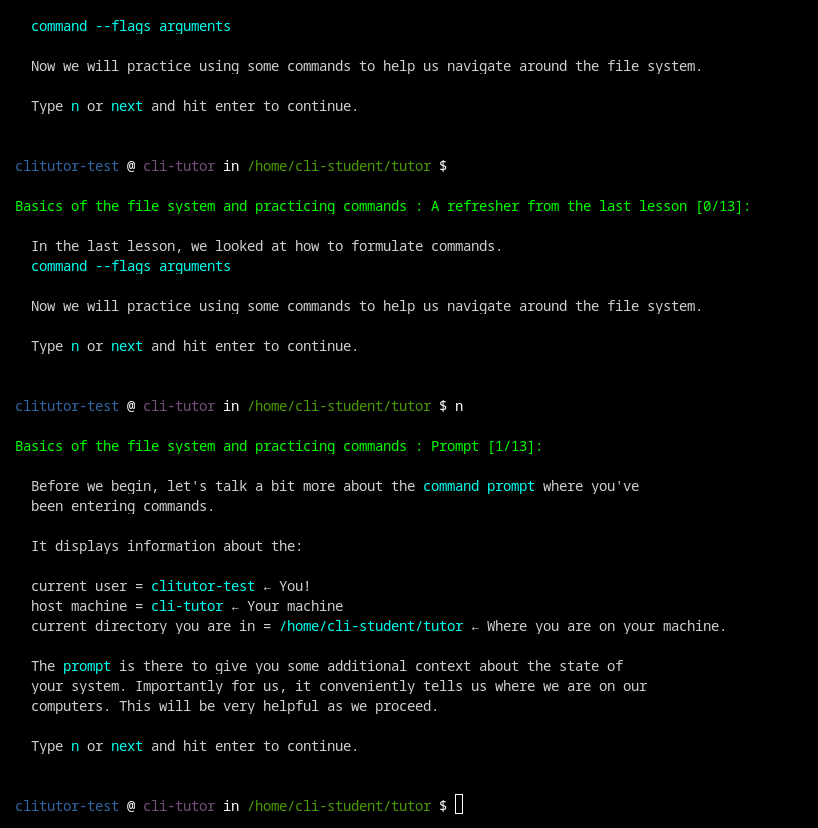
\includegraphics[width=1\textwidth]{img/cliexpansionfull}
	\caption{Screen shot of a \textit{CLI-Tutor} lesson showing values interpolated into the lesson.}
	\label{fig:webversion}
\end{figure}


